\documentclass[12pt,a4paper,twoside,openright]{report}
\usepackage{algpseudocode}		% ambienti per la scrittura di algoritmi
\usepackage{algorithm}			% 

\usepackage{epsfig}			% figure eps
\usepackage{graphicx}			% figure qualsiasi
\usepackage{amsmath,amsfonts,amsthm}	% package di scrittura matematica
\usepackage{amssymb}
\usepackage{psfrag}
\usepackage{fancyhdr}
\usepackage{url}
\usepackage{array}
\usepackage{subfigure}
\usepackage{lscape}
\usepackage{colortbl}
\usepackage{alltt}
\usepackage{tabularx}
\usepackage[english]{babel}
\usepackage[nottoc]{tocbibind}
\sloppy
\raggedbottom

\linespread{1.3}
\renewcommand{\baselinestretch}{1.3}

\makeatletter
\def\cleardoublepage{\clearpage\if@twoside \ifodd\c@page\else
\hbox{}
\vspace*{\fill}
\begin{center}
%This page intentionally contains only this sentence.
\end{center}
\vspace{\fill}
\thispagestyle{empty}
\newpage
\if@twocolumn\hbox{}\newpage\fi\fi\fi}
\makeatother

%\newcites{wb}{Web References}

%------------------------------------------------------
% Impostazioni per il controllo sillabazione vedove/orfane ect..
%
% \looseness=1 o \looseness=-1 prima di un paragrafo per
% allungarlo o accorciarlo di una riga
%------------------------------------------------------

\lefthyphenmin=4
\righthyphenmin=4
\tolerance=1000
\hyphenpenalty=100
\emergencystretch=1 cm

\widowpenalty=5000
\clubpenalty=2500



%--------------------------------------------------------
% impostazioni per la dimensione delle pagine
%--------------------------------------------------------
\renewcommand{\headrulewidth}{0.5pt}
\hoffset=-15mm
%\topmargin=0mm
\headheight=15pt
\textwidth=140mm
\headsep=5mm
\voffset=-5mm
%\hsize=13cm
%\textwidth=164mm
\textheight=230mm
\evensidemargin=25mm
\oddsidemargin=25mm
%\marginparwidth=0mm

\renewcommand{\abovecaptionskip}{0pt}
\renewcommand{\belowcaptionskip}{0pt}
%--------------------------------------------------------------
%impostazione headers
%--------------------------------------------------------------

\pagestyle{fancy}
%\addtolength{\headwidth}{\marginparsep}
%\addtolength{\headwidth}{\marginparwidth}
\renewcommand{\chaptermark}[1]{\markboth{#1}{}}
\renewcommand{\sectionmark}[1]{\markright{\thesection\ #1}}
\fancyhf{}
\fancyfoot[LE,RO]{\bfseries\thepage}
\fancyhead[RO]{\bfseries\rightmark}
\fancyhead[LE]{\bfseries\leftmark}
\fancypagestyle{plain}{%
\fancyhead{} % get rid of headers
\fancyfoot{}
\renewcommand{\headrulewidth}{0pt} % and the line
}


\newenvironment{myverse}
{\small}
{}

\newenvironment{myabstract}{%
  \begin{center}%
    \null\vfil
    \bfseries \abstractname
  \end{center}}%
{\par\vfil\null}

\begin{document}

\pagenumbering{roman}
\setcounter{page}{1}
\pagestyle{empty}

%--------------------------------------------------------------------------------
% include la pagina del titolo
%--------------------------------------------------------------------------------
%\linespread{1}
\begin{titlepage}
\vspace*{-2.5cm}
\bfseries
\begin{center}
  \LARGE
  Politecnico di Milano\\
  \Large
  Facolt\`{a} di Ingegneria dell'Informazione\\


\psfig{file=images/logopm,width=4cm}

\begin{large}
Corso di Laurea in Ingegneria Informatica\\
Dipartimento di Elettronica e Informazione\\
\end{large}

\vspace{1.0cm}
\begin{Large}
\dots Titolo della tesi \dots\\
\dots al massimo su due righe \dots
\end{Large}  
\end{center}
\vspace*{5.5cm}
\large
\begin{flushleft}
\hspace{-2cm}  Relatore: \dots nome del relatore\\
\hspace{-2cm}  Correlatore: \dots eventuale correlatore\\
\end{flushleft}
\vspace*{1.5cm}

\hspace{1cm}
\parbox{14cm}{
    \begin{tabular}{lll}
        Tesi di Laurea di: & Nome COGNOME     & matr. XXXXXX\\
                           & Nome COGNOME     & matr. XXXXXX\\
    \end{tabular}
}




\vspace*{1.5cm}
\begin{center}



  Anno Accademico 20XX-20XX



\end{center}
\end{titlepage}
\cleardoublepage

%--------------------------------------------------------------------------------
% dedica
%--------------------------------------------------------------------------------
\thispagestyle{empty}

\begin{flushright}
\Large\textit{dedica\dots}
\end{flushright}

%\null\vfil

\cleardoublepage

%--------------------------------------------------------------------------------
% ringraziamenti
%--------------------------------------------------------------------------------
\thispagestyle{empty}

\chapter*{Ringraziamenti}
Ringraziamenti vari, massimo una o due pagine.

\begin{flushleft}
Milano, 1 Aprile 2005
\end{flushleft}

\begin{flushright}
\emph{\dots nome \dots}
\end{flushright}

\cleardoublepage
\thispagestyle{empty}

\pagestyle{fancy}
\renewcommand{\contentsname}{Table of Contents}%

%--------------------------------------------------------------------------------
% sommario riassuntivo in italiano
%--------------------------------------------------------------------------------
\chapter*{Sommario}
Se la tesi \`e  scritta in Inglese, deve essere incluso un sommario introduttivo in Italiano. Nel sommario devono essere riassunti tutti i contenuti della tesi. Di fatto, il sommario in Italiano pu\`o essere la semplice traduzione del primo capitolo introduttivo della tesi, di cui mantiene l'eventuale struttura a sezioni.

\section*{Prima sezione}
\dots

\section*{Seconda sezione}
\dots

\section*{Organizzazione}
Questa tesi \`e organizzata come segue. 
\begin{itemize}
\item Nel Capitolo \ref{chap:one} \dots
\item Nel Capitolo \ref{chap:two} \dots
\item Nel Capitolo \ref{chap:three} \dots
\item \dots
\end{itemize}
La tesi si conclude con il Capitolo \ref{chap:conclusions}. Sono
discussi i risultati ottenuti e sono presentati alcuni possibili
sviluppi futuri.


\section*{Contributi}
Questo lavoro si distingue per i seguenti contributi originali:
\begin{itemize}
\item \dots riassunto sintetico dei diversi contributi
\item \dots
\item \dots
\end{itemize}


%--------------------------------------------------------------------------------
% indice
%--------------------------------------------------------------------------------
\tableofcontents
\cleardoublepage

\pagenumbering{arabic}

\setcounter{page}{1}

%--------------------------------------------------------------------------------
% introduzione
%--------------------------------------------------------------------------------
\chapter{Introduction}
\label{chap:one}
Introduzione al lavoro. Inizia direttamente, senza nessuna sezione.

Argomenti trattati suddivisi sezione per sezione\dots

Per citare un articolo, ad esempio \cite{Ackley1987} o \cite{Ackley1987,Altenberg1994} utilizzare il comando \texttt{\\cite}. 

Per gestire i file di tipo \texttt{bib} esiste il programma \texttt{JabRef} disponibile sul sito \texttt{http://jabref.sourceforge.net/}.

\section*{Original Contributions}
This work include the following original contributions:
\begin{itemize}
\item \dots riassunto sintetico dei diversi contributi
\item \dots
\item \dots
\end{itemize}

\section*{Outline of the Thesis}
This thesis is organized as follows: 
\begin{itemize}
\item In Chapter~\ref{chap:one} \dots
\item In Chapter~\ref{chap:two} \dots
\item In Chapter~\ref{chap:three} \dots
\item \dots
\end{itemize}
Finally, in Chapter~\ref{chap:conclusions}, \dots




\chapter{\dots}
\label{chap:two}
\section{Introduction}
Introduzione agli argomenti trattati nel capitolo, dalle 4 alle 10 righe.

\section{\dots}
Argomenti trattati suddivisi sezione per sezione\dots

\section{Figure}
Per includere delle figure come la Figura~\ref{fig:figura} 
usare il comando \texttt{\\includegraphics}.

%--------------------------------------------------------------------------------
% esempio di inclusione immagine
%--------------------------------------------------------------------------------
\begin{figure}[tbh]
  \centering
  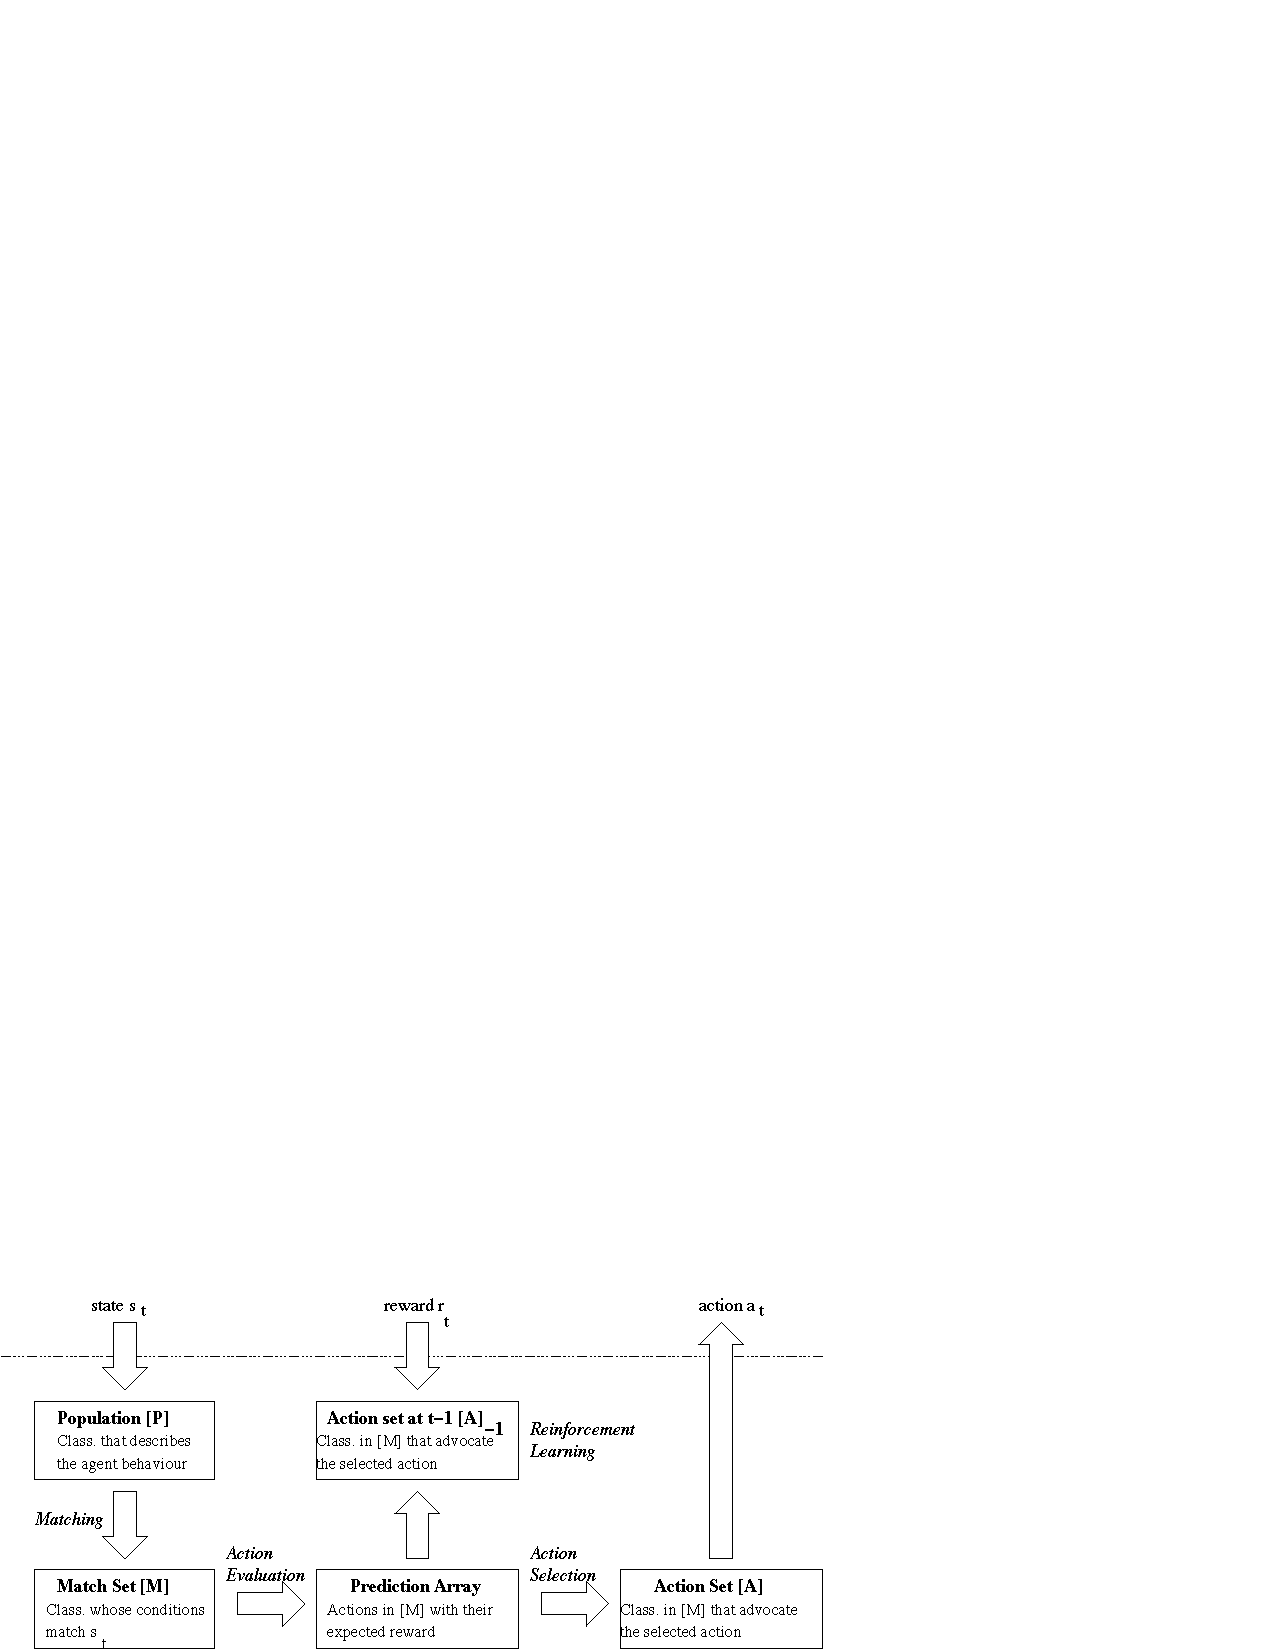
\includegraphics[scale=0.7]{images/esempio}
  \caption{\dots titolo}
  \label{fig:figura}
\end{figure}

\section{Algoritmi}
Per includere degli algoritmi come l'Algoritmo~\ref{alg:esempio}
usare lo stile \texttt{algpseudocode} presente nel package~\texttt{algorithmicx}.

%--------------------------------------------------------------------------------
% esempio di algoritmo
%--------------------------------------------------------------------------------
\begin{algorithm}[t]
  %%%
%%%
%%%	the Q-learning algorithm
%%%
%%%
\begin{algorithmic}[1]
\State Initialize $Q(\cdot,\cdot)$ arbitrarily
\ForAll{episodes}
   \State $t$ $\leftarrow$ 0
   \State Initialize $s_{t}$
   \Repeat
      \State $a_{t} \gets \pi(s_{t})$
      \State perform action $a_{t}$; observe $r_{t+1}$ and $s_{t+1}$
      \State $Q(s_{t},a_{t}) \gets Q(s_t,a_t) + \alpha( r_{t+1} + \gamma \max_{a\in A} Q(s_{t+1},a) -  Q(s_t,a_t))$
      \State $t \gets t+1$
   \Until{$s_{t}$ is terminal}
\EndFor
\end{algorithmic}

  \caption{Un esempio di algoritmo.}
  \label{alg:esempio}
\end{algorithm}


\section{Summary}

Riassunto del capitolo

\chapter*{\dots aggiungere capitoli a volont\`a}



%--------------------------------------------------------------------------------
% conclusioni e direzioni future
%--------------------------------------------------------------------------------
\chapter{Conclusions and Future Works}
\label{chap:conclusions}
Conclusioni del lavoro e sviluppi futuri. Massimo una o due pagine.

%--------------------------------------------------------------------------------
% appendici
%--------------------------------------------------------------------------------
\part*{Appendices\label{part:app}\addcontentsline{toc}{part}{Appendices}}
\appendix
\chapter{\dots}
\label{app:one}
\section{Introduction}
Introduzione agli argomenti trattati nell'appendice, dalle 4 alle 10 righe.

\section{\dots}
Argomenti trattati suddivisi sezione per sezione. 
Alla fine del capitolo non includere alcun sommario.



\chapter{\dots}
\label{app:two}
\section{Introduction}
Introduzione agli argomenti trattati nell'appendice, dalle 4 alle 10 righe.

\section{\dots}
Argomenti trattati suddivisi sezione per sezione. 
Alla fine del capitolo non includere alcun sommario.


\bibliographystyle{plain}
\bibliography{tesi.bib}
\end{document}
